\section{Intro}

What is mass? Mass is kind of energy.


Course goals:
\begin{enumerate}
	\item Pleasure of lecturer 
	\item Recognize definitions in mechanics
	\item Recognize physical ideas
\end{enumerate}
 Energy is a conserved value as a result of time symmetry.
 
 
 \section{Mechanics}
 
 Movement of bodies
 
Galileo Galilei (1564-1642)

Nicolaus Copernicus (1473-1543)

Isaac Newton (1642-1727)

$\:$ Johannes Kepler

$\:$ Tycho Brahe

Albert Einstein
\subsection{vectors}
Vector is variable with value and direction.
\begin{itemize}
	\item  $\vec{A}$ - vector A
	\item  $\mid \vec{A} \mid$ or $A$ -  value of vector
	\item  $\hat{A}$  - unit vector in direction of $A$
\end{itemize}
\paragraph{Vector sum}
Both of vectors must be same unit.
$\vec{A}+\vec{B}$

\begin{center}
	\includegraphics[width=0.3\linewidth]{./lect1/pic1.png}
\end{center}

$\vec{A}+\vec{B}=\vec{A}+\vec{B}$ - Commutativity

\paragraph{Vector subtraction}

$$\vec{A}-\vec{B}=\vec{A}+(-\vec{B})$$

$-\vec{B}$ - opposite direction

$$\vec{A}+\vec{B}=-(\vec{A}+\vec{B})$$
\paragraph{Vector sum of multiple vectors} Order isn't important!
$\vec{A}+(\vec{B}+\vec{C})=(\vec{A}+\vec{B})+\vec{C}$ - Associativity

\begin{center}
	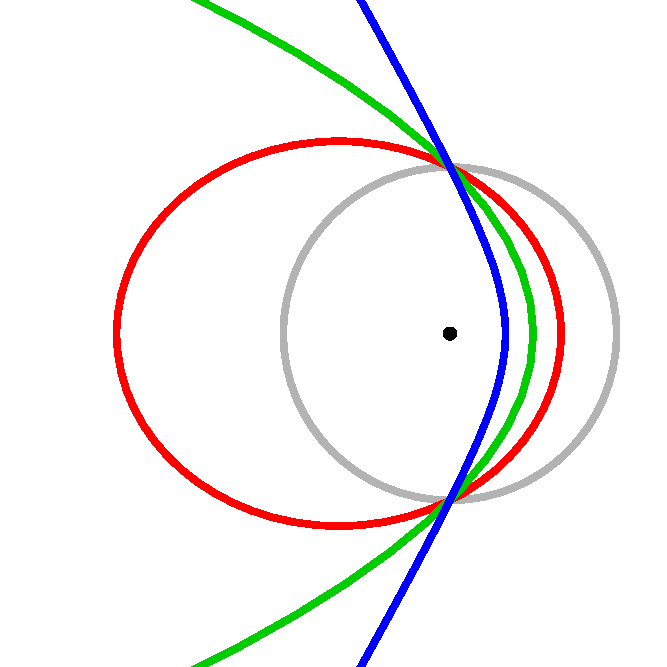
\includegraphics[width=0.3\linewidth]{./lect1/pic2.png}
\end{center}
\paragraph{Multiplication by scalar}
$k \cdot (\vec{A}+\vec{B})=k\cdot\vec{A}+k\cdot\vec{B}$ - Distributive

A physical quantity must fulfill following conditions to be a vector: 
\begin{enumerate}
	\item To have value and direction independent on coordination system
	\item Satisfy parallelogram law of vector sum (Commutativity)
\end{enumerate}
%$\vec{F}=(12N) \cdot (-\hat{y})$

\paragraph{Counter example to 2:}
Define turn of $90\degree$ around an axis according to right hand.
Turn around x and then y is not equal to turn y and then x. 
$\vec{A}+\vec{B}\neq\vec{A}+\vec{B}$
\paragraph{Vector multiplication} Don't have to be same unit.
\begin{enumerate}
	\item Scalar multiplication (dot product, inner product) - result is scalar. For $\vec{A}, \vec{B}$ with $\angle\vec{A}\vec{B}=\theta$ then $\vec{A}\cdot\vec{B}=\vec{B}\cdot\vec{A}=AB\cos\theta$.
	Product of vector A on projection of vector B on it.

\begin{center}	
	\includesvg[eps,svgpath = lect1/,width=0.2\linewidth]{pic3}
\end{center}
	
	For perpendicular vectors scalar product is $0$.
	
		Using components (Cartesian coordinate system):
		Define unit vector and axis($x,y,z$). Take vector $\vec{A}$ with angle $\theta$ to $x$.
		Take projection of $\vec{A}$ on axis: $A_x,A_y,A_z$. Then $\vec{A}=A_x\hat{x}+A_y\hat{y}+A_z\hat{z}$.
		
		$$\vec{A}\cdot\hat{x}=(A_x\hat{x}+A_y\hat{y}+A_z\hat{z})\cdot\hat{x}=A_x\hat{x}\cdot\hat{x}+A_y\hat{y}\cdot\hat{x}+A_z\hat{z}\cdot\hat{x}=A_x + 0 + 0 = A_x$$
		$$A=\sqrt{\vec{A}\cdot\vec{A}}=((A_x\hat{x}+A_y\hat{y}+A_z\hat{z})\cdot(A_x\hat{x}+A_y\hat{y}+A_z\hat{z}))^\frac{1}{2}=\sqrt{A_x^2 + A_y^2 + A_z^2}$$
		$$\hat{A}=\frac{\vec{A}}{\mid \vec{A} \mid}=\frac{A_x}{\mid \vec{A} \mid}\cdot\hat{x}$$
		$$\vec{A} \cdot \vec{B} = A_xB_x + A_yB_y$$
		$$\hat{A} \cdot \hat{B} = \frac{\vec{A}}{A} \cdot \frac{\vec{B}}{B} = \frac{\vec{A} \cdot \vec{B}}{A\cdot B} = \frac{AB\cos \alpha}{AB} = \cos \alpha$$
	\item Vector product (cross product) - $\vec{A} \times \vec{B}$
	
	$$\vec{C} = \vec{A} \times \vec{B} = -\vec{B} \times \vec{A}$$
	$$\vec{C} = \hat{c}AB\sin\alpha$$
	
	\subparagraph{Right hand rule:}
	
	Four fingers in direction of shortest path between $\vec{A}$ and $\vec{B}$, then thumb shows direction of $\vec{C}$.

\begin{center}	
	\includesvg[eps,svgpath = lect1/,width=0.2\linewidth]{pic4}
\end{center}
	
	$$\vec{A} \times \vec{A} = 0$$	
	$$\vec{A} \times(\vec{B} + \vec{C}) =  \vec{A} \times\vec{B} + \vec{A} \times\vec{C}$$
	
\end{enumerate}